\subsection{Flöde genom en vägg vid transient förlopp}

%To regerenate the figures use /code/pdesolver/calculateRisetime.m
%with the argument /code/pdesolver/wallstep.mat

För att visualisera hur flödet genom en vägg förändras med
förändringar i vädret utomhus modelleras ett tidssteg där utomhustemperaturen förändras från 0 till $\unit[10]{^\circ C}$. Inomhustemperaturen hålls konstant till $\unit[20]{^\circ C}$. Detta har gjorts för en vägg utan och en vägg med isolering, se figur \ref{fig:energyflow_trans}. Beräkningarna är genomförda med finita elementmetoden där den oisolerade väggen består av $\unit[0,5]{m}$ tegel och den isolerade har dessutom $\unit[0,1]{m}$ mineralull.

Falltiden för dessa två väggar beräknades till $\unit[34,8]{timmar}$ för väggen utan isolering respektive $\unit[98,8]{timmar}$ för väggen med isolering. 
Värt att notera är också att det tog $\unit[9,6]{timmar}$ respektive $\unit[16,8]{timmar}$ för energiflödet att falla $\unit[10]{\%}$. 

\begin{figure}[hpbt]
\centering

\subfloat[Energiflöde ut från insidan av en oisolerad vägg.]{
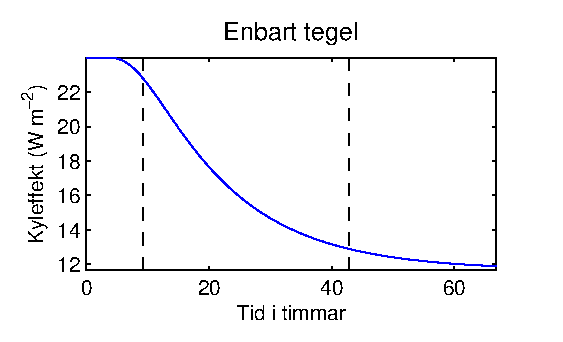
\includegraphics[width=6cm]{images/noinsulationstep.eps}
}\vspace{5mm}
\subfloat[Energiflöde ut från insidan av en isolerad vägg]{
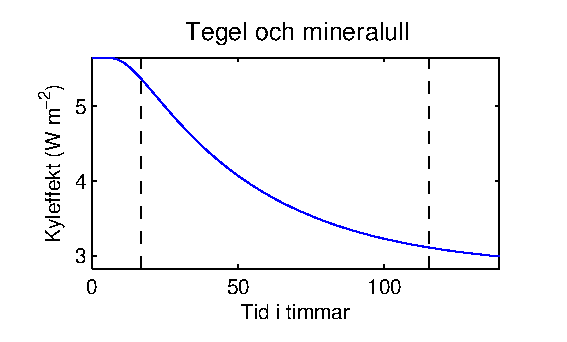
\includegraphics[width=6cm]{images/insulationstep.eps}
}

\subfloat[\emph{\color{red} Energiflödet från insidan av burspråket. Tio procents fall
kom så tidigt som efter $45,52$ minuter och hela fallet (dvs mellan strecken) på $169,22$ minuter}]{
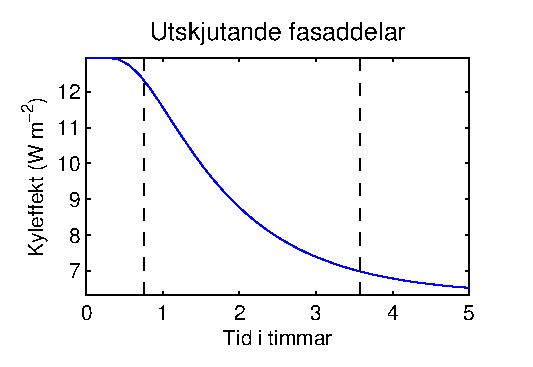
\includegraphics[width=6cm]{images/baywallstep.eps}
}
\caption{\label{fig:energyflow_trans} Energiflödet ut från insidan av en vägg. Vid tiden $t<0$ råder jämviktsläge med $\unit[0]{^\circ C}$ på utsidan och $\unit[20]{^\circ C}$ inomhus. Utomhustemperaturen förändras vid tiden $t=0$ i ett steg till $\unit[10]{^\circ C}$. De streckade linjerna markerar $\unit[10]{\%}$ stigning och $\unit[90]{\%}$ stigning.}

\end{figure}

Här kan alltså ses en avsevärd skillnad i hur lång tid det tar innan väggen har anpassat sig till en ny temperatur. En sådan här plötslig och drastisk förändring i temperaturen är inte något som sker speciellt ofta och ju kortare dagarna är destå mindre är temperaturvariationerna mellan dag och natt. \cite{SMHItempskillnad}
Vid nyår kan man inte förvänt sig en skilland på mer än $\unit[2-3]{^\circ C}$. Vi kan ändå konstatera att förändringen i temperatur fortplantar sig betydligt långsammare i en isolerad vägg än en oisolerad. Har man då väggar som är olika bra isolerade behöver man troligen även ha två olika reglersystem för de delar av huset som ligger närmast respektive vägg, om man inte reglerar enbart efter inomhustemperaturen. 

Återigen visas det att en isolerad vägg är mer motståndskraftig för förändringar i utomhustemperaturen vilket är en fördel om ett jämt inomhusklimat eftersträvas.
